%!TEX root = ../thesis.tex

\section{QDDモータの採用}
オフィス環境においてロボットアームが人や物に被害を与えないことは極めて重要である.本研究ではロボットアームが人や物と衝突した時の衝撃を軽減することを目的として,QDD(Quasi Direct Drive)モータを採用する.QDD モータは,低減速比で高いバックドライバビリティを有し,優れた応答性を示す点が特徴である.いくつかの研究では,QDDモータを適切に制御することで,衝突時の衝撃を軽減することが示されている.

飯塚ら\cite{飯塚浩太2021}は,DDモータに10:1の減速機構を組み合わせたQDDモータを用いた柔軟な3自由度ロボットアーム(図\ref{fig:3DofArm}参照)を開発し,その評価実験を行っている.同研究では,制御周波数を高めることで制御ゲインを向上させることを確認しており,柔軟性と剛性の切り替えが自在に行えることを示している.

また,Gealyら\cite{gealy2019}が開発したBlue(図\ref{fig:blue}参照)では,アームの関節にQDDモータを採用することで,高いバックドライバビリティと応答性を活かした作業を可能にしている.特に,動作中に人間が接触した場合でも,関節が柔軟に動作する特性や,人間が遠隔操作を行い,コーヒーメーカを操作や,机拭き作業などを行えることを示している\cite{Blue:online}.

さらに,Zhaoら\cite{10106520}は,モバイルプラットフォームへの搭載を視野に入れた軽量ロボットアームを開発している(図\ref{fig:qddarm}参照).同アームは6自由度や7自由度のロボットアームが多い中,5自由度で構成されており,部品の形状,素材によって軽量化を図っている.同アームはピックアンドプレースタスクを想定した実験により,高い柔軟性と安全性を実証している.

これらの研究から,QDDモータを適切に制御することで,衝突時の衝撃を軽減することが確認されている.一方で,QDDモータを使用したオープンソースロボットアームは確認されていない.また,QDDモータをロボットアームに活用した事例は少なく,QDDモータの技術的なノウハウや応用可能性については,まだ十分に探求されていないのが現状である.

\begin{figure}[h]
  \centering
  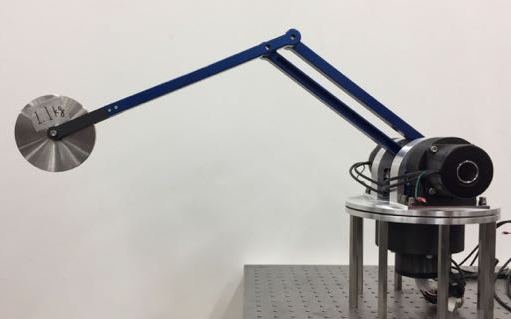
\includegraphics[width=10cm]{images/haikei/3DofArm.png}
  \caption[3-DoF robot arm using QDD motor]{3-DoF robot arm using QDD motor (source: \cite{飯塚浩太2021})}
  \label{fig:3DofArm}
\end{figure}
\begin{figure}[h]
  \centering
  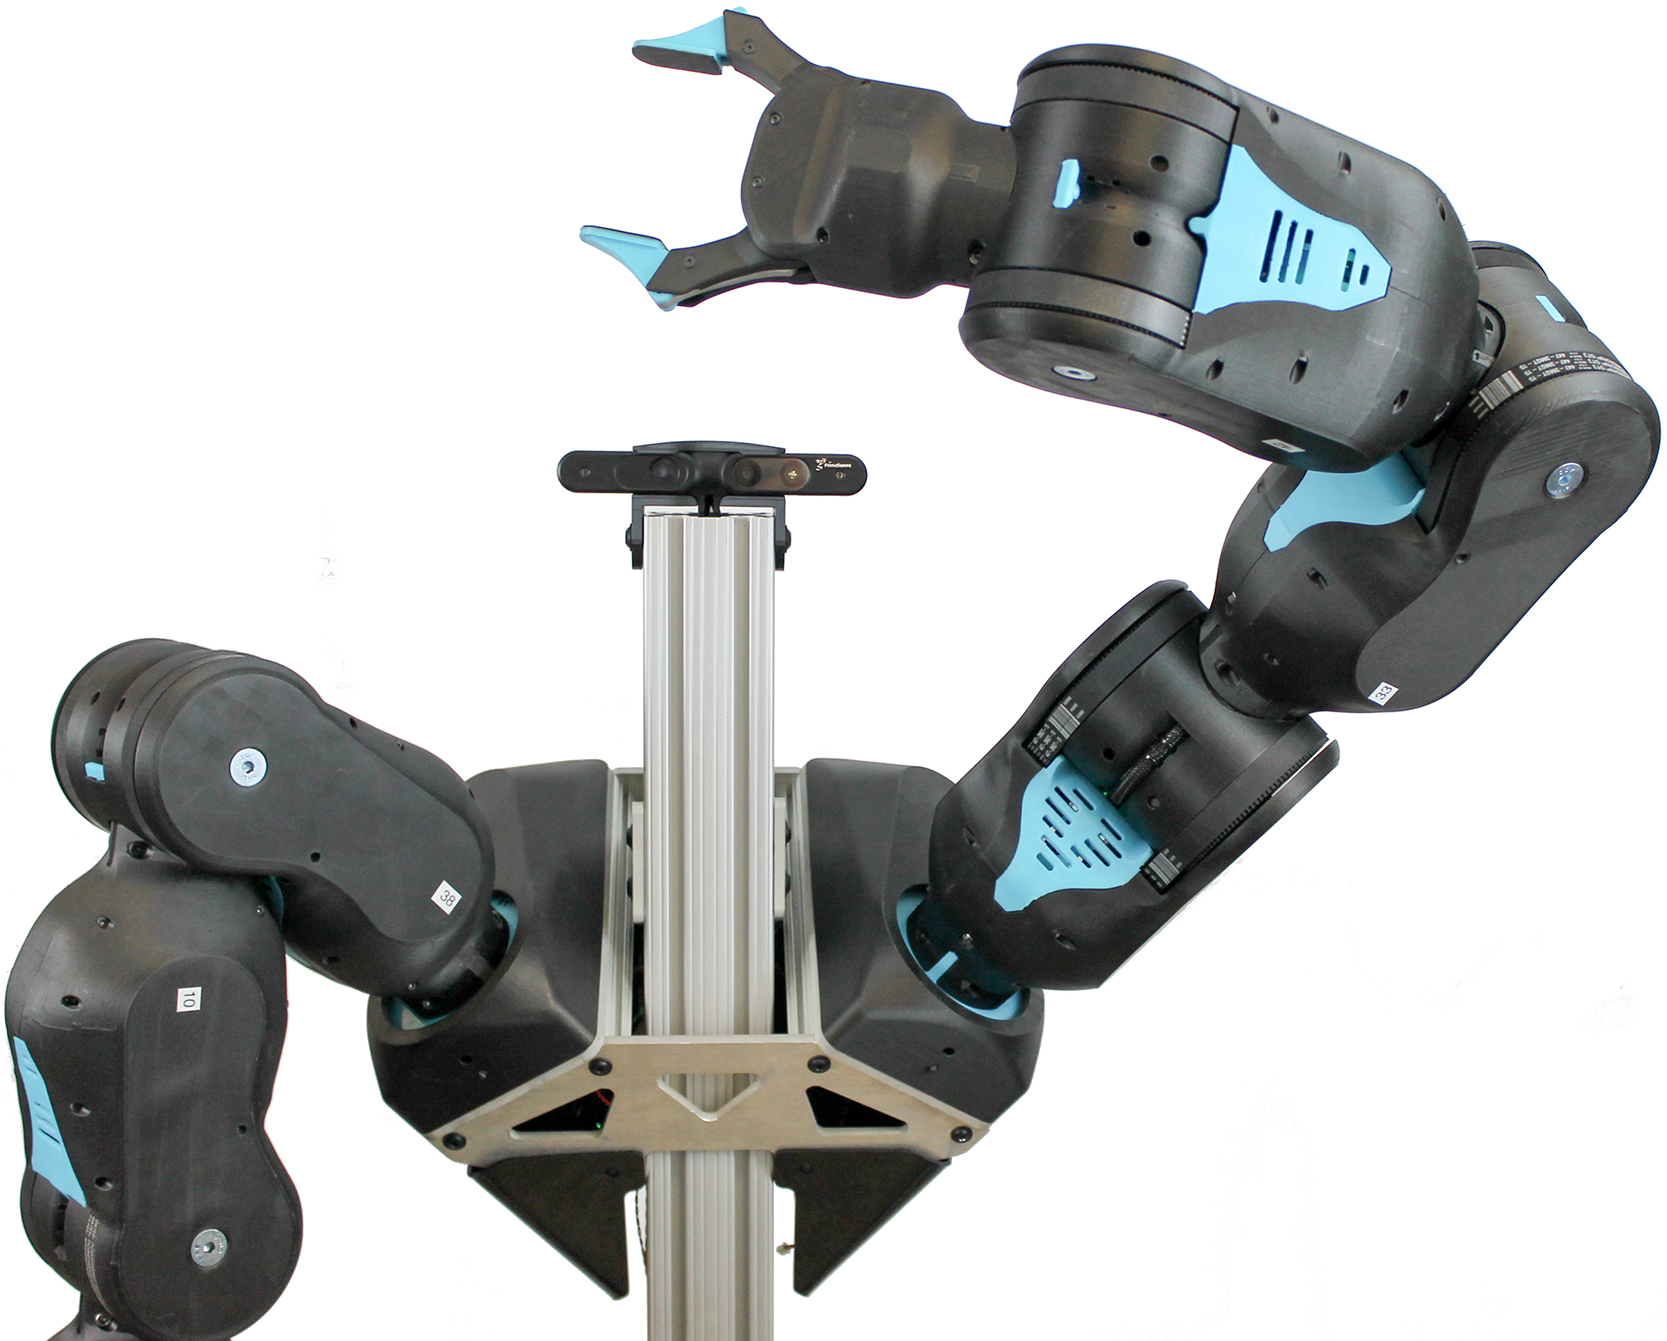
\includegraphics[width=10cm]{images/haikei/twoArmTeaser.jpg}
  \caption[The Blue robot using QDD motor]{The Blue robot using QDD motor (source: \cite{Blue:online})}
  \label{fig:blue}
\end{figure}
\begin{figure}[h]
  \centering
  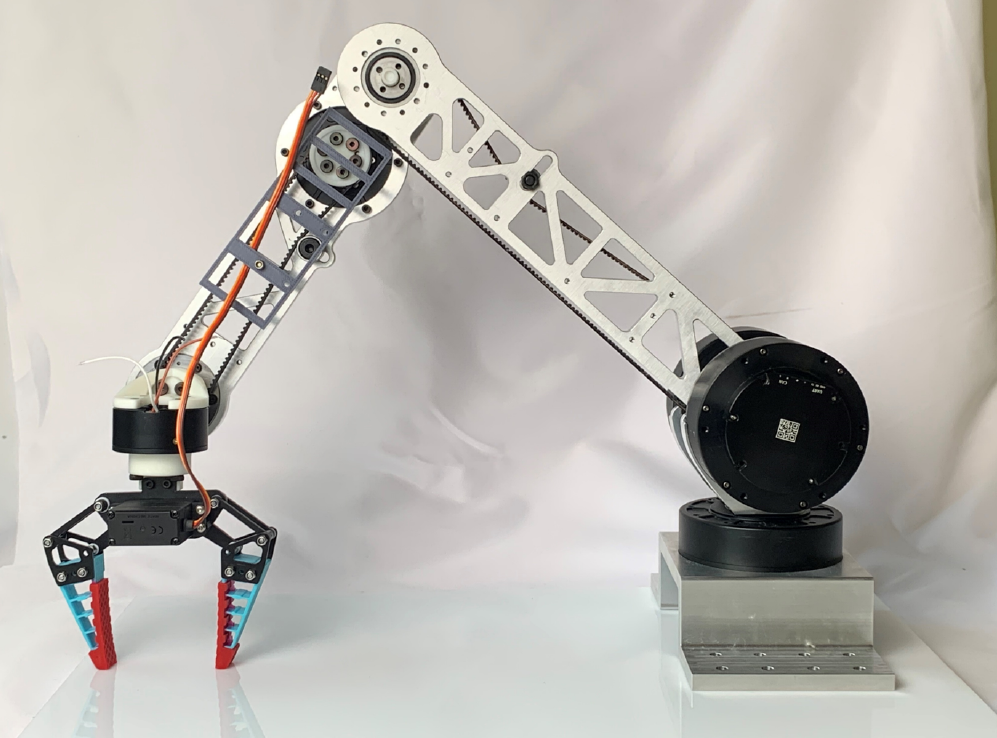
\includegraphics[width=10cm]{images/haikei/qddarm.png}
  \caption[The proposed 5-DOF articulated quasi-direct drive (QDD) robot arm,
  together with a commercial 1-DOF soft gripper]{The proposed 5-DOF articulated quasi-direct drive (QDD) robot arm,
  together with a commercial 1-DOF soft gripper (source: \cite{10106520})}
  \label{fig:qddarm}
\end{figure}
\clearpage